\DiaryEntry{Inside Interesting Integrals, Feynman's Trick (Chap 3)}{2022-03-21}{Integrals}

We consider a definite integral where (i) the limits depend on a parameter $\alpha$ and (ii) the integrand is parametrized by $\alpha$ as well,

\bee
I(\alpha) = \int_{a(\alpha)}^{b(\alpha)} f(x, \alpha) dx
\eee

Differentiating with respect to $\alpha$ yields (shown without proof here)

\begin{equation}\label{2022-03-21:eq1}
\boxed{
\frac{d I(\alpha)}{d \alpha} = \int_{a(\alpha)}^{b(\alpha)} \frac{ \partial f(x, \alpha) }{\partial \alpha } dx + f(b, \alpha) \frac{db}{d \alpha} - f(a, \alpha) \frac{da}{d \alpha}
}
\end{equation}

The first term comes from exchanging the integral (with respect to $x$) with the derivative (with respect to $\alpha$). The second and third term come from considering the integral change when the upper and lower term vary, respectively.

Let's start with a simple example with constant limits and $f(\alpha, x) = \alpha x$. We can calculate the integral directly as

\bee
I(\alpha) = \int_{a}^{b} \alpha x dx = \left. \frac{\alpha x^2}{2} \right|_a^b = \frac{\alpha (b^2 - a^2)}{2}
\eee

Taking the derivative yields

\bee
\frac{d I(\alpha)}{d \alpha} = \frac{b^2 - a^2}{2}
\eee

Let's calculate the derivative directly by using \eqref{2022-03-21:eq1} (we have used the fact that the limits are constant),

\bee
\frac{d I(\alpha)}{d \alpha} = \int_{a}^{b} \frac{ \partial f(x, \alpha) }{\partial \alpha } dx = \int_{a}^{b} \frac{ \partial \alpha x}{\partial \alpha } dx = \int_{a}^{b} x dx = \frac{b^2 - a^2}{2}
\eee

and this corresponds to the result obtained via direct calculation. \qed

Next we have a non-constant upper limit and we apply \eqref{2022-03-21:eq1},

\bee
I = \int_0^t ax dx \quad \frac{dI}{dt} = f(b,\alpha) \frac{db}{d \alpha} = at \cdot 1 = at
\eee

When the upper limit changes from $t$ to $t + \Delta t$, the area (integral value) changes by $at$. Direct evaluation yields $I = at^2/2$ and $dI/dt = at$. \qed

While these examples were certainly interesting, the real power of \eqref{2022-03-21:eq1} lies in solving new integrals (by introducing a parameter to existing integrals and then taking the derivative); e.g.

\bee
\int_0^\infty \frac{1}{x^2 + a^2} dx = \frac{1}{a} \left. \arctan \frac{x}{a} \right|_0^\infty = \frac{\pi}{2a}
\eee

Applying \eqref{2022-03-21:eq1} yields

\bee
\int_0^\infty \frac{-2a}{(x^2 + a^2)^2} dx = (-1) \frac{\pi}{2a^2}
\eee

which we simpliy to

\bee
\boxed{
\int_0^\infty \frac{a}{(x^2 + a^2)^2} dx = \frac{\pi}{4a^2}
}
\eee

We can check the value using scipy / integrate as in the following.

\begin{verbatim}
import numpy as np
import scipy.integrate as int

a=1.0

def f(x):
    return(a/(x**2+a**2)**2)

int.quad(f, 0, 100)
>>> (0.7853978301041107, 4.1516289119382996e-11)
    
np.pi/(4*a**2)
>>> 0.7853981633974483
\end{verbatim}

\qed


Also interesting is

\bee
I = \int_0^{\pi/2} \sin ax dx = \frac{1-\cos a \pi/2}{a}, \quad \frac{dI}{da} = \frac{\cos(a\pi/2) - 1}{a^2} + \frac{\pi \sin(a\pi/2)}{2a}
\eee

Differentiating yields

\bee
\frac{dI}{da} = \int_0^{\pi/2} \frac{d}{da}\sin ax dx = \int_0^{\pi/2} x \cos ax dx
\eee

and therefore

\bee
\boxed{
\int_0^{\pi/2} x \cos ax dx = \frac{\cos(a\pi/2) - 1}{a^2} + \frac{\pi \sin(a\pi/2)}{2a}
}
\eee

Interestingly, \eqref{2022-03-21:eq1} also works without integration bounds; i.e.

\bee
\boxed{
\frac{d I(\alpha)}{d \alpha} = \int \frac{ \partial f(x, \alpha) }{\partial \alpha } dx 
}
\eee

From this we deduce

\bee
\boxed{
\int x \cos ax dx = \frac{a x \sin{\left( a x\right) }+\cos{\left( a x\right) }}{{{a}^{2}}}
}
\eee

as $I(a) = \int \sin ax dx = - \frac{\cos ax}{a}, \frac{dI(a)}{da} = \int \frac{d \sin ax}{da} = \int x \cos ax dx$ and \\ $\frac{- d \frac{\cos ax}{a}}{da} = \frac{a x \sin{\left( a x\right) }+\cos{\left( a x\right) }}{{{a}^{2}}}$.

Also fun is the case $a=1$ with

\bee
\int x \cos x dx = x \sin x +\cos a x
\eee

We have sneaked in a parameter $a$ to get the integration going and finally removed it via setting $a=1$ :-) The integrand $x \cos x$ is shown in the following Figure.

\begin{figure}[H]
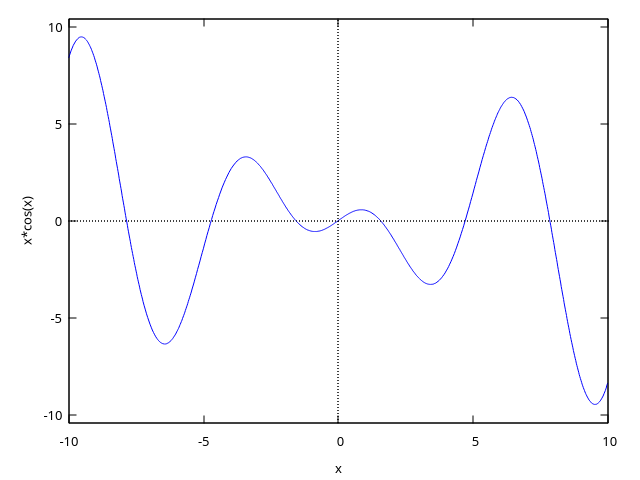
\includegraphics[scale=0.7]{images/2022-03-21_plot_1.png}
\end{figure}
    

\subsection{Normal Distribution}

Now, let's use the machinery in earnest and try the following integral,

\bee
I = \int_{- \infty}^\infty e^{-\frac{x^2}{2}} dx
\eee

We consider the integral over the right interval and introduce

\bee
g(t) = \left( \int_{0}^t e^{-\frac{x^2}{2}} dx \right)^2
\eee

Our original integral then becomes

\bee
I = \int_{- \infty}^\infty e^{-\frac{x^2}{2}} dx = 2 \sqrt{g(\infty)}
\eee

Let's apply \eqref{2022-03-21:eq1} to calculate $dg/dt$ (note that the only thing that varies is the upper limit and we therefore have only the $f(b, \alpha) \frac{db}{d \alpha}$ term),

\bee
\frac{dg}{dt} = 2 \left( \int_{0}^t e^{-\frac{x^2}{2}} dx \right) \frac{d}{dt} \left( \int_{0}^t e^{-\frac{x^2}{2}} dx \right)
= 2 \left( \int_{0}^t e^{-\frac{x^2}{2}} dx \right) e^{-\frac{t^2}{2}} = 2 \int_{0}^t e^{-\frac{x^2 + t^2}{2}} dx
\eee

Next we make a variable substitution $y = x/t \rightarrow x = yt \rightarrow dx = t dy$ and arrive at

\bee
\frac{dg}{dt} = 2 \int_{0}^1 t e^{-\frac{y^2 t^2 + t^2}{2}} dy = 2 \int_{0}^1 t e^{-\frac{t^2 (1 + y^2)}{2}} dy
\eee

The whole purpose of the substitution is that we can express the integrand as derivative as follows,

\bee
2 t e^{-\frac{t^2 (1 + y^2)}{2}} = \frac{\partial}{\partial t} \left( - \frac{2 e^{-\frac{t^2 (1 + y^2)}{2}} }{1+y^2} \right)
\eee

and therefore

\bee
\frac{dg}{dt} = \int_{0}^1 \frac{\partial}{\partial t} \left( \frac{2 e^{-\frac{t^2 (1 + y^2)}{2}} }{1+y^2} \right) = -2 \frac{d}{dt} \int_{0}^1 \frac{e^{-\frac{t^2 (1 + y^2)}{2}} }{1+y^2} dy
\eee

We can integrate this expression with respect to $t$ and obtain

\be\label{2022-03-21:eq2}
g(t) = -2 \int_{0}^1 \frac{e^{-\frac{t^2 (1 + y^2)}{2}} }{1+y^2} dy + C
\ee

where $C$ is the (important) integration constant. In the definition of $g(t)$ we set $t=0$ and then

\bee
g(0) = \left( \int_{0}^t e^{-\frac{x^2}{2}} dx \right)^2 = 0
\eee

Now we set $t = 0$ in $\int_{0}^1 \frac{e^{-\frac{t^2 (1 + y^2)}{2}} }{1+y^2} dy$ which yields $\int_{0}^1 \frac{1}{1+y^2} dy = \left. \arctan y \right|_0^1 = \frac{\pi}{4}$. We can combine things at $t=0$ and obtain

\bee
g(0) = 0 = -2 \frac{\pi}{4} + C \rightarrow C = \frac{\pi}{2}
\eee

and so

\bee
g(t) = -2 \int_{0}^1 \frac{e^{-\frac{t^2 (1 + y^2)}{2}} }{1+y^2} dy + \frac{\pi}{2}
\eee

We are interested in $I = 2 \sqrt{g(\infty)}$, therefore

\bee
g(\infty) = -2 \lim_{t \rightarrow \infty} \int_{0}^1 \frac{e^{-\frac{t^2 (1 + y^2)}{2}} }{1+y^2} dy + \frac{\pi}{2}
\eee

For increasing $t$, the integrals gets "peakier" and in the limit becomes zero; therefore $g(\infty) = \frac{\pi}{2}$, from which follows

\bee
\sqrt{g(\infty)} = \sqrt{\frac{\pi}{2}} \rightarrow I = 2 \sqrt{g(\infty)} = 2 \sqrt{\frac{\pi}{2}} = \sqrt{2 \pi}
\eee

and we arrive at

\bee
\boxed{
I = \int_{- \infty}^\infty e^{-\frac{x^2}{2}} dx = \sqrt{2 \pi}}
\eee




%%% Local Variables:
%%% mode: latex
%%% TeX-master: "journal"
%%% End:
